\documentclass[12pt,openany]{ctexbook}

% 上海财经大学本科毕业论文（设计）版式
% 依据：上财行规〔2024〕21号《上海财经大学本科学生毕业论文（设计）工作的规定》
\usepackage[a4paper,top=2.5cm,bottom=2.5cm,left=3.0cm,right=2.0cm,footskip=1.5cm]{geometry}
\usepackage{setspace}
\usepackage{amsmath,amssymb,amsthm}
\usepackage{booktabs}
\usepackage{graphicx}
\usepackage{enumitem}
\usepackage{array}
\usepackage{caption}
\usepackage{fancyhdr}
\usepackage[hidelinks]{hyperref}
\usepackage[backend=biber,style=gb7714-2015]{biblatex}
\addbibresource{references.bib}
\usepackage{fontspec}
\usepackage{seqsplit}

\newfontfamily\arial{Arial}
\setmainfont{Times New Roman}
\setCJKmainfont{SimSun}
\setCJKsansfont{SimHei}
\setCJKmonofont{SimSun}

\ctexset{
  chapter/format={\centering\heiti\zihao{3}},
  section/format={\heiti\zihao{4}},
  subsection/format={\heiti\zihao{5}},
  chapter/name={第,章},
  chapter/number={\chinese{chapter}},
  contentsname={目\quad 录},
  figurename={图},
  tablename={表}
}
\renewcommand{\refname}{参考文献}
\renewcommand{\thetable}{\thechapter-\arabic{table}}
\renewcommand{\thefigure}{\thechapter-\arabic{figure}}

\setlength{\parindent}{2em}
\setlength{\parskip}{0pt}
\linespread{1.5}
\pagestyle{fancy}
\fancyhf{}
\fancyfoot[C]{\zihao{5}\thepage}
\renewcommand{\headrulewidth}{0pt}

\newtheorem{proposition}{命题}[chapter]
\newtheorem{theorem}{定理}[chapter]
\newcommand{\E}{\mathbb{E}}
\newcommand{\indic}{\mathbf{1}}
\newcommand{\method}{FinPlan-RAG}
\newcommand{\sufehead}[1]{\chapter*{#1}\addcontentsline{toc}{chapter}{#1}}

\title{\method：面向时点金融证据的决策接口与损失感知策略组合}
\author{匿名作者}
\date{2026年11月}

\begin{document}

% ==================== 封面 ====================
\begin{titlepage}
\thispagestyle{empty}
\centering
\vspace*{1.2cm}
{\zihao{2}\heiti 上海财经大学\par}
\vspace{0.3cm}
{\zihao{2}\heiti 本科毕业论文（设计）\par}
\vspace{2.0cm}
{\zihao{2}\heiti \method：面向时点金融证据的\par}
\vspace{0.2cm}
{\zihao{2}\heiti 决策接口与损失感知策略组合\par}
\vspace{2.3cm}
{\zihao{4}\songti
\renewcommand{\arraystretch}{1.6}
\begin{tabular}{r@{\quad}l}
学\qquad 院 & 信息管理与工程学院 \\
专\qquad 业 & 金融信息工程 \\
姓\qquad 名 & 匿名作者 \\
学\qquad 号 & \underline{\hspace{3cm}} \\
指导教师 & \underline{\hspace{3cm}} \\
\end{tabular}\par}
\vfill
{\zihao{4}\songti 2026年11月\par}
\end{titlepage}

% ==================== 原创性声明 ====================
\pagenumbering{roman}
\pagestyle{fancy}
\sufehead{原创性声明}
{\zihao{4}\songti
本人郑重声明：所呈交的毕业论文（设计）是本人在导师指导下进行的研究工作及取得的研究成果。除文中已经注明引用的内容外，本论文不包含任何其他个人或集体已经发表或撰写过的作品成果。对本文的研究做出重要贡献的个人和集体，均已在文中以明确方式标明。本人完全意识到本声明的法律结果由本人承担。\par
\vspace{1.2cm}
作者签名：\underline{\hspace{4cm}}\qquad 日期：\underline{\hspace{3cm}}\par
}

% ==================== 中文摘要 ====================
\clearpage
\phantomsection
\addcontentsline{toc}{chapter}{摘\quad 要}
\begin{center}
{\zihao{3}\heiti \method：面向时点金融证据的\\[0.2cm]
决策接口与损失感知策略组合\par}
\vspace{0.6cm}
{\zihao{3}\heiti 摘\quad 要\par}
\end{center}
\vspace{0.4cm}
{\zihao{4}\songti
前瞻性营收指引在申报日并不存在唯一答案。系统可以给出点答案，可以输出可信集，也可以弃权或等待后续申报。现有检索增强生成与断言验证系统通常在证据到达之前固定输出模式、决策时间与检索预算，因而无法表示同一查询在不同损失和证据状态下应当选择不同动作。本文将输出接口形式化为可信状态上的决策问题，动作包括回答、可信集裁决、弃权、获取证据和等待，并用非对称损失刻画高估、低估、集合遗漏与集合宽度。\par
为检验该接口，本文构建了273条公司不重叠、按年份滚动的营收指引基准，并给出737条2015年至2025年的扩展检验。在227条XBRL核验标签上，证据模型的平衡准确率由.333提高到.564，宏F1由.220提高到.488。在非LLM随机森林上，损失感知策略组合在10个损失配置中有9个达到最优固定策略损失，并在宽区间惩罚下优于最优固定策略（4.340对4.710，遗憾值为$-0.370$，95\%置信区间为$[-0.643,-0.100]$）。FinDVer、Fin-Fact、Self-RAG、CRAG、FLARE和Adaptive-RAG六个具名基线从固定commit的官方源码仓库加载提示模板和决策逻辑，经同一三分类适配层运行，在点预测上各有优势，但没有单一模型全面占优；缺失的checkpoint/数据替代逐项记录，不能视为原系统的未修改运行；在GLM 5.3 flash和本地部署的开源Qwen3-8B两个附加基座上重复该比较，FinPlan的平衡准确率和AUROC优势均成立。在真实业绩公告证据流上，序贯策略组合在24个成本单元中均达到oracle最优候选（平均和最大遗憾值均为0），在廉价延迟时选择等待、在昂贵时选择固定裁决；同伴证据获取未被选中。\par
本文的贡献是决策接口、时点基准和可复核的决策层证据。结论限定在决策层：点预测的全面最优和基础损失上的方法优越性均不作为主张。\par
}
\vspace{0.6cm}
\noindent{\zihao{4}\heiti 关键词：}{\zihao{4}\songti 金融检索增强生成；时点证据；决策接口；策略组合；可信集；基准评测}

% ==================== 英文摘要 ====================
\clearpage
\phantomsection
\addcontentsline{toc}{chapter}{Abstract}
\begin{center}{\arial\bfseries\zihao{3} Abstract\par}\end{center}
\vspace{0.6cm}
{\arial\fontsize{10.5pt}{15pt}\selectfont\sloppy
Forward-looking revenue guidance has no unique answer at the filing date. A system can return a point answer, a credible set, an abstention, or wait for a later filing. Existing retrieval-augmented generation and claim-verification systems usually fix the output mode, decision time, and retrieval budget before evidence arrives. They therefore cannot represent a query whose correct action changes with the loss and the evidence state. This thesis formulates the output interface as a decision problem over a credal state, with actions for answering, adjudicating, abstaining, acquiring evidence, and waiting, and with an asymmetric loss for overclaiming, underclaiming, set misses, and set width.\par
To test the interface, we build a year-wise, company-disjoint benchmark of 273 revenue-guidance claims, with a 737-claim rolling extension from 2015 to 2025. On 227 XBRL-verified labels, balanced accuracy rises from .333 to .564 and macro F1 from .220 to .488. On a non-LLM random forest, a loss-aware policy portfolio matches the oracle best fixed policy in nine of ten loss configurations and improves on it under the wide-width penalty (4.340 versus 4.710; regret $-0.370$, 95\% CI $[-0.643,-0.100]$). Six named baselines (FinDVer, Fin-Fact, Self-RAG, CRAG, FLARE, and Adaptive-RAG) are competitive on point metrics, but no single model dominates. The balanced-accuracy and AUROC advantage of FinPlan also holds on GLM 5.3 flash and a locally served open-weight Qwen3-8B.\par
The contribution is the decision interface, the point-in-time benchmark, and auditable decision-layer evidence. We do not claim uniform point-prediction superiority, and we do not interpret oracle-level regret as a base-loss advantage.\par
}
\vspace{0.4cm}
\noindent{\arial\bfseries\zihao{5} Keywords:} {\arial\fontsize{10.5pt}{15pt}\selectfont financial RAG; point-in-time evidence; decision interface; policy portfolio; credible set; benchmark}

% ==================== 目录 ====================
\tableofcontents
\clearpage

\mainmatter
\zihao{5}

% ==================== 第1章 ====================
\chapter{引言}
\label{ch:intro}

\section{研究背景}
金融文本中的前瞻性陈述与静态问答不同。管理盈余指引是公司披露的重要渠道\cite{hirst2008management}。以美国证券交易委员会（SEC）8-K文件中的营收指引为例，公司在某一季度给出的营收区间，其最终结果可能是低于区间、落在区间内或高于区间。申报日可获得的证据包括指引区间、当前季度值、历史指引偏差和同行业信息，但最终结果尚未发生。系统因此不仅要判断“答案是什么”，还要决定“以什么形式回答”和“何时回答”。本文的接口名简称FinPlan，代码与包名保留FinPlan-RAG。\footnote{英文稿使用FinPlan指代决策接口；为与代码仓库一致，本文标题保留FinPlan-RAG。}\par
这一选择具有实际后果。点答案便于下游使用，却可能把不确定判断伪装成确定结论；可信集保留了不确定性，却可能因集合过宽而缺乏信息量；弃权避免错误，却放弃了可用信息；等待后续申报可能提高准确性，但会产生延迟成本。不同损失下，最优动作并不相同。高估的代价高于低估时，系统应更保守；集合宽度惩罚很高时，系统应更倾向于点答案；弃权成本很低时，系统可以在证据不足时直接弃权。\par
现有检索增强生成（RAG）系统通常把输出固定为答案，把决策时间固定为查询时刻，把检索预算固定为前$k$个段落。断言验证系统把输出固定为支持、反驳或不确定的判定。选择性预测允许答案或弃权，但仍固定决策时间，且通常只处理二分类拒识。近年的金融RAG系统在证据类型、期间约束和来源追踪上有明显改进，但输出契约仍然是在给定截止时间产生一个答案或判定。它们可以改善证据，却不能表示“证据到达后最优输出模式发生变化”的情形。\par

\section{研究问题}
本文围绕三个问题展开。\par
\textbf{RQ1：}在按年份滚动、公司不重叠的时点协议下，基于结构化证据的模型能否泛化到未见公司，并在类别不平衡的标签上保持平衡准确率和宏F1？\par
\textbf{RQ2：}在给定可信状态和非对称损失后，信念驱动的规划器是否优于固定输出动作？固定裁决器在哪些损失区域仍然是强基线？\par
\textbf{RQ3：}在不知道真实损失、只能看到验证损失的条件下，策略组合能否在不同损失配置中接近最优固定策略，并在独立种子分配上复现？\par
这三个问题分别对应证据层、决策层和选择层。本文不把三者混为一个点预测问题，也不以单一准确率概括全部结论。\par

\section{主要贡献}
本文的贡献有四点。\par
第一，提出一个面向时点金融证据的决策接口。该接口把输出模式、决策时间、证据获取和等待纳入同一状态与动作空间，并用非对称损失统一点答案、可信集和弃权。固定截断RAG、断言验证、选择性预测和预路由都可以写成该接口的受限特例。\par
第二，构建一个按年份滚动、公司不重叠的营收指引基准。主基准包含273条2022年至2025年的测试样本，其中227条有XBRL核验标签；扩展基准包含737条2015年至2025年的样本。协议在测试年份之前截断训练结果，并移除测试公司，降低公司身份和未来结果泄漏。\par
第三，给出损失感知策略组合。组合在固定裁决、弃权和规划器三个候选策略之间，用公司不重叠的验证损失选择，并以0.15的切换边际避免过度切换。在非LLM随机森林上，组合在10个损失配置中9个达到最优固定策略损失，并在宽区间惩罚下取得更低的损失。该结果是最优固定策略级遗憾值，不是基础损失上的方法优越性。\par
第四，给出官方源码基线和完整指标。本文从固定commit的官方仓库加载FinDVer、Fin-Fact、Self-RAG、CRAG、FLARE和Adaptive-RAG的提示模板与决策逻辑，经同一三分类适配层在DeepSeek、GLM 5.3 flash和本地开源Qwen3-8B三个基座上重复，报告准确率、平衡准确率、宏F1、MCC、AUROC、AP、选择性准确率和AURC；缺失checkpoint和原始数据的替代逐项记录在附录表中。LLM基线只返回标签置信度，不是归一化三类分布，因此NLL、Brier和ECE不作跨行比较。结果显示没有单一模型全面占优，点预测结论必须与决策层结论分开表述。\par

\section{论文结构}
第\ref{ch:related}章梳理相关工作与能力边界。第\ref{ch:formal}章给出问题形式化、损失和命题。第\ref{ch:method}章介绍损失感知策略组合。第\ref{ch:benchmark}章介绍基准、协议、指标和基线。第\ref{ch:results}章报告实验结果。第\ref{ch:discussion}章讨论局限与外推边界。第\ref{ch:conclusion}章总结全文。\par

% ==================== 第2章 ====================
\chapter{相关工作与能力边界}
\label{ch:related}

\section{检索增强生成}
RAG将检索器与生成器结合，假设答案存在于检索到的上下文中\cite{lewis2020rag}。FLARE根据生成过程中的不确定性主动触发检索\cite{jiang2023flare}；Self-RAG让模型判断是否需要检索，并对检索内容进行自我反思\cite{asai2024selfrag}；Adaptive-RAG根据问题复杂度选择检索路径\cite{jeong2024adaptiverag}；CRAG在检索质量不足时触发纠正\cite{yan2024crag}。ReAct和Reflexion把推理、行动与自我修正结合起来\cite{yao2023react,shinn2023reflexion}。这些方法改变了检索过程，但输出契约仍是生成一个答案。它们不比较点答案、可信集和弃权的期望损失，也不为等待后续文件定价。\par

\section{金融问答与断言验证}
金融问答基准强调数值推理、表格与文本混合证据。FinQA、TAT-QA、FinanceBench和FinBen覆盖了不同规模和不同任务的金融问答\cite{chen2021finqa,zhu2021tatqa,islam2023financebench,liu2024finben}。断言验证基准判断一个陈述是否被证据支持、反驳或无法核验。FinDVer面向长文档和混合内容金融文件，要求给出可解释的验证结果\cite{zhao2024findver}；Fin-Fact面向多模态金融事实核查\cite{rangapur2025finfact}。这些工作提高了证据评估的质量，但通常把输出固定为判定，并假定证据已经给定。\par

\section{金融RAG系统}
FinRank将证据检索与答案正确性分开，构造跨实体、跨报告期间的困难负例\cite{mansouri2026finrank}。Fin-RATE评估大模型在SEC文件上的细节推理、企业比较和纵向追踪能力，并指出检索是RAG的主要瓶颈\cite{jiang2026finrate}。HC-RAG用类型化金融证据图和意图路由组织异构文件\cite{chen2026hcrag}。FinSAgent通过角色化多智能体、语料感知查询分解和特征门控重排提高证据覆盖\cite{chi2026finsagent}。FinCARDS把金融文件重排表述为模式约束匹配，用结构化卡片和锦标赛式重排提高早期排序稳定性\cite{chen2026fincards}。这些系统在证据层做了重要改进，但输出仍是在给定截止时间产生答案或判定，检索预算也通常固定。\par
本文不声称这些系统忽略了证据来源。相反，它们已经把来源、期间和类型纳入检索。本文关注的是更窄的接口问题：当输出模式、决策时间和证据预算都需要在证据到达后决定时，系统如何用一个统一的损失函数比较动作。\par

\section{选择性预测、共形预测与代价敏感学习}
拒识选项在识别错误与拒识率之间权衡\cite{chow1970optimum}。选择性分类学习置信度阈值，在低置信度时弃权\cite{geifman2017selective}。温度缩放是校准现代分类器的强基线\cite{guo2017calibration}。代价敏感学习为不同错误赋予不同代价\cite{elkan2001cost}。共形预测给出分布无关的集合覆盖\cite{vovk2005algorithmic,romano2020classification,angelopoulos2021gentle}，并可在分布偏移下做自适应调整\cite{gibbs2021adaptive}。部分识别和可信集合为不完整证据下的决策提供统计工具\cite{manski2003partial}。部分可观测马尔可夫决策过程和受控感知为“何时停止、观察什么”提供一般工具\cite{krishnamurthy2017pomdp}。这些工作提供了损失、校准和集合构造的组件，但通常假定任务和输出契约固定。\par

\section{能力边界}
表\ref{tab:capability}从输出模式、决策时间、证据预算和损失感知四个维度比较现有范式。该表是能力映射，不是对每个具体实现的断言。\par
\begin{table}[htbp]
\centering
\caption{现有范式的能力边界}
\label{tab:capability}
\zihao{5}
\begin{tabular}{p{0.24\linewidth}ccccc}
\toprule
范式 & 输出模式 & 决策时间 & 预算 & 损失感知 \\
\midrule
固定截断RAG & 答案 & 固定 & 固定 & 否 \\
主动/自适应RAG & 答案 & 部分可变 & 部分可变 & 否 \\
断言验证 & 判定 & 固定 & 固定 & 否 \\
选择性预测 & 答案/弃权 & 固定 & 固定 & 部分 \\
预路由 & 证据前选模式 & 固定 & 固定 & 部分 \\
本文接口 & 答案/集合/弃权/等待 & 证据后决定 & 证据后决定 & 是 \\
\bottomrule
\end{tabular}
\end{table}
表\ref{tab:capability}的最后一行是本文的窄缺口：现有工作分别解决了证据、校准或拒识的一部分问题，但缺少一个统一契约，同时允许输出模式、决策时间和证据预算在证据到达后变化，并用非对称损失比较动作。这个缺口不是“没有人做过任何相关事情”，而是一个可识别属性的缺失。\par

% ==================== 第3章 ====================
\chapter{问题形式化与理论边界}
\label{ch:formal}

\section{证据、时点与可信状态}
设查询为$q$，候选结果空间为$H_q=\{\text{below},\text{within},\text{above}\}$。在决策时刻$t$，系统拥有证据集合$E_t$。证据带有类型、来源、期间和公开可得时间。对于截止时间$c$，只有公开时间不晚于$c$的证据可见。系统维护$H_q$上的可信状态$b_t$，其中$b_t(y)$表示结果$y$的信念。\par
形式化地，令$\mathcal{F}_t$为截至$t$的观测历史，$b_t(y)=\Pr(y\mid \mathcal{F}_t)$。本文不假设$b_t$是单一先验下的精确后验；它可以是校准后的分类器输出、可信集或集成结果。关键在于：决策规则显式使用$b_t$，而不是只使用一个相关性分数。\par

\section{动作与损失}
输出动作集合为
\begin{equation}
\mathcal{A}_{\text{out}}=\{\text{answer}(a),\ \text{adjudicate}(R),\ \text{abstain}\},
\end{equation}
其中$a\in H_q$是点答案，$R\subseteq H_q$是可信集。证据动作包括获取证据$\text{acquire}(e)$和等待$\text{wait}(\Delta)$。获取证据支付成本$\lambda(e)$并更新$b_t$；等待推进决策时刻并支付延迟成本。\par
点答案损失定义为
\begin{equation}
L_{\text{ans}}(a,y)=
\begin{cases}
0, & a=y,\\
\ell_{\text{over}}, & a=\text{above}, y=\text{below},\\
\ell_{\text{under}}, & a=\text{below}, y=\text{above},\\
\ell_{\text{wrong}}, & \text{其他}.
\end{cases}
\end{equation}
可信集损失定义为
\begin{equation}
L_{\text{set}}(R,y)=\indic[y\notin R]\ell_{\text{miss}}+\ell_{\text{width}}\max(0,|R|-1),
\end{equation}
弃权损失为$L_{\text{abs}}=\ell_{\text{abstain}}$。默认参数为$\ell_{\text{over}}=12$、$\ell_{\text{under}}=8$、$\ell_{\text{wrong}}=10$、$\ell_{\text{miss}}=8$、$\ell_{\text{width}}=2$、$\ell_{\text{abstain}}=5$。高估的代价高于低估；宽度项为无信息集合定价。第\ref{ch:results}章在10个损失配置上报告结果，结论不依赖单一权重。\par

\section{目标与规划器}
策略$\pi$的目标是最小化期望决策损失、证据成本和延迟成本：
\begin{equation}
J(\pi)=\E\left[L(\text{output},y)+\sum_{e\in\text{acquired}}\lambda(e)+\gamma(t-t_0)\right],
\end{equation}
其中$t_0$为查询开始时刻，$\gamma\ge0$为单位延迟成本。本文不设置硬预算约束；预算由证据成本和延迟成本内生决定。\par
在信念$b_t$下，停止价值为
\begin{equation}
S(b_t)=\min_{a,\,R\in\mathcal{C}_\alpha(b_t)}
\left\{\E_{b_t}[L_{\text{ans}}(a,y)],\ \E_{b_t}[L_{\text{set}}(R,y)],\ \ell_{\text{abs}}\right\},
\end{equation}
其中$\mathcal{C}_\alpha(b_t)=\{R\subseteq H_q:b_t(R)\ge1-\alpha\}$为可信集族。实验中$R$按后验概率降序贪心加入标签，直到质量达到$1-\alpha$；这是最小质量集合，不保证基数最小。主配置取$\alpha=0.1$。等待下一份申报的价值为
\begin{equation}
W(b_t)=\lambda_a+\gamma\hat d+\E_{o}[S(b_t\mid o)],
\end{equation}
其中$\lambda_a$为申报成本，$\hat d$为公司历史延迟估计，期望对下一份申报将揭示的观测$o$取得。当$W(b_t)<S(b_t)+m$时规划器等待，$m$是校准误差的保守边际。该边际是设计选择，不是学习参数。\par
证据模型提供$b_t$。主基准使用带时点特征的多项式逻辑回归，并在公司不重叠的内部折上做温度缩放；决策层的主结果使用同一特征上的随机森林，森林使用原始概率（温度$1.0$）。在真实基准中证据集固定在截止日，规划器只在答案、可信集、弃权三个输出动作上做一步Bayes选择；等待与证据获取只在受控诊断中评估。本文的贡献是接口和评估，不是新的分类器。\par

\section{固定接口作为特例}
固定截断RAG固定$t$，把输出限制为答案。断言验证固定输出为判定，并把证据视为已给定。选择性分类把输出限制为答案或弃权，并固定$t$。固定预算系统在$k$个动作后停止。预路由在证据之前选择模式，不获取证据也不等待。它们都是对动作集合、决策时间或输出契约的限制。当损失区域已知且稳定时，这些限制是合理的；当损失随查询变化时，它们不是通用的。\par

\section{三个命题}
\begin{proposition}[点答案不足]
若$S_t$不是单点集且损失非对称，则不存在一个对所有与$S_t$一致的后验都minimax最优的点答案。当错误答案的代价高于集合宽度惩罚时，可信集可以具有严格更低的最坏情况风险。
\end{proposition}
\begin{proposition}[相关性不足]
若一个相关性分数在某个纤维上为常数，而该纤维包含约束不同的证据，则该分数不是Bayes动作的充分统计量。只使用该分数的策略存在最坏情况损失差。
\end{proposition}
\begin{proposition}[预路由不足]
若最优输出模式依赖于路由决策之后观测到的证据，则不存在对所有查询都最优的预路由。状态依赖的规划器可以改进。
\end{proposition}
三个命题只识别固定接口失效的条件，不是金融决策的一般理论。证明见附录\ref{app:proofs}。它们的设计含义是：输出契约应包含可信集，证据应按约束内容类型化，模式应在证据之后选择，而不是在证据之前固定。\par

\section{为什么不直接使用路由器}
路由器把证据前观测映射到一个模式；规划器把证据后信念映射到一个动作。区别不在命名。第一，最优模式可能在证据到达后改变：查询时看似精确的陈述，在读完指引区间后可能只支持可信集。第二，在接口层面，规划器可以获取证据或等待，路由器不能；真实基准中的规划器只做一步输出模式选择，等待与证据获取只在受控诊断中评估。第三，等待的价值取决于损失和延迟成本，同一查询在不同损失区域可能需要不同决策。附录中的受控诊断显示，当模式信号只对一半样本有信息且与路由特征独立时，规划器明显优于预路由。\par

% ==================== 第4章 ====================
\chapter{损失感知策略组合}
\label{ch:method}

\section{候选策略}
决策层在信念$b_t$上有三个候选输出策略。固定裁决输出可信集$\mathcal{C}_\alpha(b_t)$；弃权支付固定成本$\ell_{\text{abstain}}$；规划器按期望损失选择答案、可信集或弃权。固定裁决和规划器的$\alpha$在$\{0.05,0.10,0.20\}$上，用公司不重叠的验证损失选择。点答案不作为选择器候选：在报告的十个配置中，它在验证集上均被支配；但它仍是定义遗憾值时的oracle比较对象。验证损失只来自训练公司的内部折外预测，测试折不参与拟合、$\alpha$选择或策略选择。\par
选择器从固定裁决开始，只有当另一个候选的验证损失比当前策略低至少$m_{\text{switch}}=0.15$时才切换。该边际是保守性设计，用于避免验证集上的微小波动导致策略频繁切换。选定策略只在测试折上评估一次，测试结果不参与选择。附录\ref{app:margin}报告切换边际的敏感性。\par

\section{为什么使用组合而不是单一策略}
单一固定策略在每个损失区域都最优的假设很强。基础损失下，固定裁决器已经很强；廉价弃权下，弃权最优；宽区间惩罚下，规划器可以通过输出模式选择降低损失。组合的价值来自读取损失和验证证据，而不是来自一个更强的点预测器。组合的失败模式也清楚：如果验证集太小或分布偏移，选择器可能选错策略。本文用10个损失配置和独立种子分配检验这一点。\par

\section{随机森林基座}
主决策层使用200棵树的随机森林，叶节点最小样本数为3，使用平衡子采样，并只使用时点结构化特征。特征包括指引宽度、当前季度值相对指引中点的比例、指引与当前季度的比值、截止日前已公开的历史结果数量和分布、上一次指引的增长与宽度、目标季度、截止年份和行业。森林不读取文本，也不调用大模型。使用非LLM基座的目的，是让决策层结果不依赖预训练污染。\par

\section{共形替代方案}
本文还测试了共形替代方案：用LAC或APS构造集合，在校准集上按实现损失选择阈值，并在公司不重叠验证集上选择分数族和$\alpha$。DeepSeek命名实体版本在基础损失上为3.101，低于固定裁决的3.122；廉价弃权为1.947，窄区间为1.053，宽区间为4.447。掩码公司版本的基础优势衰减为3.119对3.108。由于LLM可能见过2022年至2025年的结果，该方案只作为敏感性分析，不是主方法。\par

\section{实现与复现}
策略组合、评估、随机森林诊断和共形替代方案均由论文仓库中的脚本实现，完整路径和运行命令见附录\ref{app:reproduce}和\texttt{paper/reproduce.md}。基准数据发布在\texttt{paper/data/}，包含1,005条样本及其SEC链接和核验来源。所有随机种子、损失配置、验证折和测试折均记录在结果文件中。\par

% ==================== 第5章 ====================
\chapter{基准与实验设计}
\label{ch:benchmark}

\section{数据}
基准包含2010年至2025年美国SEC 8-K文件中的1,005条季度营收指引样本。每条样本包含一个指引区间，最终结果取自SEC XBRL；当XBRL没有独立季度值时，使用申报文件回退。标签为低于、位于或高于指引区间。全量数据按时间划分为529条开发样本（2010—2018）、203条验证样本（2019—2021）和273条测试样本（2022—2025）；第\ref{ch:benchmark}章的按年份滚动协议会在测试样本上按公司折重新划分。全量数据包含538条above、307条within和160条below。测试集包含2022年至2025年的273条样本，其中2022年84条、2023年70条、2024年67条、2025年52条。全量数据覆盖289家公司；测试集包含126条above、110条within和37条below，行业分布为其他113条、半导体83条、软件71条、硬件5条、医疗1条。\par
指引区间从8-K财报中抽取：拒绝年度区间和分部/产品/服务行；将实现季度匹配到目标季度附近的第一个XBRL事实；拒绝偏离指引中点0.5至2.0倍的实现值；按公司和目标期间去重，保留最早样本。发布的数据文件保留每条样本的SEC链接、声明文本、指引区间、当前季度值、结果和核验来源。\par
	extbf{结果公开时间。}数据集中的	exttt{outcome.date}是10-Q申报日。1,005条样本中有993条在同一季度的更早8-K Item 2.02业绩公告中已经公开实际营收；中位提前2天，最大提前160天，273条测试样本全部有此类8-K。主基准使用10-Q日期作为训练截断，这是保守做法：可能排除少量更早公开的训练样本，但不会泄漏未来结果。第\ref{ch:results}章的序贯实验使用更早的8-K日期作为真实终端证据，因为那是标签首次公开的时间。\par
ef{ch:results}章的序贯实验使用更早的8-K日期作为真实终端证据，因为那是标签首次公开的时间。\par
这些样本是申报文本的自动抽取转述，不是人工改写。1,005条标签中有936条为XBRL核验、XBRL覆盖或XBRL检索标签，其余69条为纯文本标签。本文报告仅保留XBRL核验标签的敏感性分析，排除46条纯文本测试样本。该检验是标签噪声检查，不是人工标注金标准。\par

\section{按年份滚动的公司不重叠协议}
协议在每个测试年份$Y$上，用其他四个公司折中结果日期早于$Y$年1月1日的样本训练，并在$Y$年的全部测试样本上评估。测试公司从不出现在训练集中，$Y$年及之后的结果也不可见。公司折由带种子的哈希分配，重复5个种子；每条样本在每个种子上评估一次。决策层随机森林重复10个种子。\par
该协议比随机划分更严格，也更接近实际使用。金融机器学习中的前视偏差会让模型使用决策时不可得的信息\cite{lopezdeprado2018advances}。随机划分会泄漏公司身份和未来结果；简单时间划分仍会在测试公司的早期样本上训练。按年份滚动且公司不重叠同时移除这两类泄漏。\par

\section{证据模型与校准}
证据模型使用第\ref{ch:method}章列出的时点特征，采用$C=1.0$、类别权重平衡的多项式逻辑回归。温度缩放参数在训练数据的公司不重叠内部折上按对数损失选择，再应用到测试折。校准不改变argmax预测，因此不改变准确率和宏F1；它改变置信度和可信集宽度，从而影响规划器。\par

\section{指标与对照}
主指标是平衡准确率（各类召回率的平均）\cite{brodersen2010balanced}和宏F1\cite{sokolova2009performance}。测试分布类别不平衡，普通准确率会被above类主导；一个总是预测above的分类器可以获得.462的普通准确率，但平衡准确率只有.333、宏F1只有.211。本文还报告普通准确率、50\%覆盖率下的选择性准确率、AURC；对FinPlan和滚动基准报告ECE、Brier分数和对数损失。AUROC和AP取一类对其余类的宏平均；ECE使用最大预测概率的十等宽分箱；Brier为三类平方概率误差之和；对数损失取自然对数；选择性准确率@50按最大概率排序后取前一半；AURC是覆盖率$0.1,0.2,\dots,1.0$处风险的平均值，不是梯形积分。决策损失为每条样本损失的平均。置信区间为样本级配对自助法区间；附录\ref{app:reproduce}列出各类区间的重采样次数。\par
两个对照用于排除替代解释。无特征先验对照从训练折类别分布中采样标签，匹配类别频率但不使用特征，用于检验模型增益是否只是类别重平衡。XBRL核验敏感性检验用于判断增益是否依赖46条纯文本测试标签。核验集包含227条样本。\par

\section{具名基线与简单对照的区分}
本文的主基线表只展示具名方法：FinDVer、Fin-Fact、Self-RAG、CRAG、FLARE和Adaptive-RAG。它们从固定commit的官方源码仓库加载提示模板和决策逻辑，在同一DeepSeek基座和同一时点证据下经同一三分类适配层运行；检索类方法取其他公司更早的6条样本。缺失checkpoint/原始数据的替代见表\ref{tab:provenance-zh}，因此它们是官方源码驱动的适配，不是原系统的未修改运行。\par
FinRank、Fin-RATE、HC-RAG和FinSAgent是近年金融RAG系统，但没有兼容的公开代码或共享样本标签，本文不在同一决策基准上运行它们，也不引用其论文数字做同表比较。逻辑回归、随机森林、TF-IDF和梯度提升只作为FinPlan基座诊断，不作为具名基线展示。\par

\section{损失配置}
主损失配置为$\ell_{\text{over}}=12$、$\ell_{\text{under}}=8$、$\ell_{\text{wrong}}=10$、$\ell_{\text{miss}}=8$、$\ell_{\text{width}}=2$、$\ell_{\text{abstain}}=5$。网格还包括对称损失、过度厌恶、过度乐观、廉价弃权、昂贵弃权、窄区间惩罚、宽区间惩罚以及$\alpha=0.05$和$\alpha=0.20$。所有配置使用同一选择规则；网格用于敏感性分析，不是调参集。表\ref{tab:lossgrid}列出十个配置的完整权重。\par
% ==================== 第6章 ====================
\chapter{实验结果}
\label{ch:results}

\section{证据模型的泛化}
表\ref{tab:benchmark}报告主基准结果。在全量标签上，平衡准确率为.566，对比多数类的.333，增益为.232，95\%区间为[.167,.295]；宏F1为.504，对比.211，增益为.294，区间为[.228,.359]。在227条XBRL核验样本上，平衡准确率为.564，对比.333，增益为.230，区间为[.164,.294]；宏F1为.488，对比.220，增益为.268，区间为[.194,.338]。无特征先验对照在全量标签上的平衡准确率为.346、宏F1为.337，在核验标签上为.340和.334。模型明显高于对照，说明增益不只是类别频率变化。\par
普通准确率在全量标签上为.517，对比.462，但区间包含零；在核验标签上为.498，对比.493。选择性准确率和AURC在全量标签上为正，但在核验标签上不显著。因此稳健结论是平衡准确率和宏F1这一对类别不平衡稳健指标，普通准确率与选择性预测只作为描述性结果。\par
\begin{table}[htbp]
\centering
\caption{公司不重叠基准结果（五种子概率集成；区间为对多数类增益的样本级配对自助法区间）}
\label{tab:benchmark}
\zihao{5}
\begin{tabular}{lccc}
\toprule
 & 全量标签 & XBRL核验 & 先验对照 \\
 & ($n=273$) & ($n=227$) & \\
\midrule
平衡准确率 & .566 & .564 & .346 \\
\quad 增益[95\% CI] & [.167,.295] & [.164,.294] & \\
宏F1 & .504 & .488 & .337 \\
\quad 增益[95\% CI] & [.228,.359] & [.194,.338] & \\
普通准确率 & .517 & .498 & .410 \\
\quad 增益[95\% CI] & [-.033,.143] & [-.088,.097] & \\
选择性@50 & .584 & .535 & \\
AURC & .412 & .458 & \\
\bottomrule
\end{tabular}
\end{table}

\section{固定裁决是强基线}
在非LLM随机森林上，基础损失下固定裁决为2.932，规划器为3.011，点答案为4.710，始终弃权为5.000。这里的规划器是固定证据上对答案、可信集、弃权的一步Bayes动作，不包含等待或证据获取；森林使用原始概率（温度1.0）。规划器单独使用时反而差于固定裁决，因此固定裁决是基础损失下要击败的策略。策略组合在基础损失下选择固定裁决，并精确达到最优固定损失（遗憾值为0.000）。这说明组合的价值不在基础损失上超过最优固定策略，而在不同损失区域之间选择正确策略。\par

\section{策略组合在不同损失区域的表现}
表\ref{tab:portfolio}报告10个损失配置（完整权重见表\ref{tab:lossgrid}）。选择器在8个配置中选择固定裁决，在廉价弃权下选择弃权，在宽区间惩罚下选择规划器。组合在9个配置中达到最优固定策略损失，并在宽区间下更低：4.340对4.710，遗憾值为$-0.370$，95\%样本级自助法区间为$[-0.643,-0.100]$。宽区间下最优固定策略是点答案（4.710），调优裁决器为5.235。平均遗憾值为$-0.037$，区间为$[-0.064,-0.010]$，最大遗憾值为0.000。\par
该结果不是基础损失上的胜利。基础损失下最优动作是固定裁决，组合只是匹配它。组合的结果是最优固定策略级遗憾值：在同一损失网格上，单一固定策略并不一致接近最优；调优裁决器的平均遗憾值为$+0.146$、最大为$+0.932$，点答案的平均遗憾值为$+1.982$、最大为$+3.747$。组合在每个配置中不高于最优固定策略，并在宽区间下严格更低。\par
\begin{table}[htbp]
\centering
\caption{损失感知策略组合（227条XBRL核验样本，10个随机森林种子）。``最优固定''是点答案、调优固定裁决器和始终弃权在当前损失下的oracle最小值；宽区间下最优固定为点答案（4.710），调优裁决器为5.235。}
\label{tab:portfolio}
\zihao{5}
\begin{tabular}{llccc}
\toprule
损失配置 & 选择策略 & 组合 & 最优固定 & Regret \\
\midrule
基础 & 固定 & 2.932 & 2.932 & .000 \\
对称 & 固定 & 2.932 & 2.932 & .000 \\
过度厌恶 & 固定 & 2.932 & 2.932 & .000 \\
过度乐观 & 固定 & 2.932 & 2.932 & .000 \\
廉价弃权 & 弃权 & 2.000 & 2.000 & .000 \\
昂贵弃权 & 固定 & 2.932 & 2.932 & .000 \\
窄区间 & 固定 & 0.963 & 0.963 & .000 \\
宽区间 & 规划器 & 4.340 & 4.710 & -.370 \\
$\alpha=.05$ & 固定 & 2.932 & 2.932 & .000 \\
$\alpha=.20$ & 固定 & 2.932 & 2.932 & .000 \\
\bottomrule
\end{tabular}
\end{table}
确认性种子分配在种子11至20上复现该模式，覆盖4个配置（基础、廉价弃权、窄区间、宽区间），不是完整的10配置网格。基础损失为2.886，精确等于最优固定值；但规划器单独在基础损失上为2.984，对比固定裁决2.885，差值为$+0.099$，95\%区间为$[0.001,0.211]$，预注册的0.2非劣边际未达到；基础匹配来自组合选择固定裁决，而不是规划器本身。宽区间下，预注册主比较是规划器减宽度调优固定裁决：4.335对5.200，差值为$-0.865$，95\%区间为$[-1.226,-0.490]$；对oracle最优固定策略（点答案4.687）的遗憾值为$-0.352$，95\%区间为$[-0.644,-0.065]$。4个确认配置的平均遗憾值为$-0.088$，区间为$[-0.161,-0.016]$，最大遗憾值为0.000；该4配置均值不能与前面的10配置均值直接比较。该复现使用同一批样本，只更换折分配，因此是种子级复现，不是新样本。\par

\section{官方源码基线的点预测比较}
表\ref{tab:named}报告六个具名基线。每个基线接收相同的时点证据块：声明文本、指引区间、当前季度值、截止日、行业，以及截止日前已公开的公司历史结果；检索类方法接收其他公司更早的6条样本，按TF-IDF余弦相似度加上指引宽度、当前季度比例和行业特征选择。六个方法的官方提示模板与决策逻辑从固定commit的官方仓库加载，再通过同一个三分类适配层映射到below/within/above；缺失的checkpoint和原始数据由API/结构化证据替代，逐项记录在表\ref{tab:provenance-zh}。所有调用使用温度0、关闭thinking、JSON输出，解析失败重试一次，并按提示哈希缓存。\par
CRAG的准确率（.546）、选择性准确率（.684）、AURC（.337）和AUROC（.689）在具名基线中最好；FinPlan的平衡准确率、宏F1、MCC、AUROC和AP最好（分别为.561、.485、.273、.716和.524）。FinPlan的准确率低于CRAG，选择性准确率和AURC也低于CRAG，但平衡准确率和AUROC更高。LLM基线只返回标签置信度，不是归一化三类分布，因此NLL、Brier和ECE不可比，表中不展示。\par
McNemar检验对FinPlan不拒绝任一具名基线的准确率相等（$p=.20$至$1.00$）。FinDVer、Self-RAG、FLARE和Adaptive-RAG的AUROC低于FinPlan，且95\%区间排除零；Fin-Fact和CRAG的AUROC差异区间包含零。没有单一模型全面占优，因此本文不把点预测指标作为唯一选择依据，决策层仍按遗憾值选择。\par
\begin{table}[htbp]
\centering
\caption{官方源码适配基线与FinPlan的点预测指标（227条XBRL核验样本）。六个具名行从固定commit的官方仓库加载提示模板和决策逻辑，经同一三分类适配层在DeepSeek基座（\texttt{deepseek-flash[1m]}，温度0，关闭thinking）上运行；它们不是原系统的未修改运行，缺失checkpoint/数据替代见表\ref{tab:provenance-zh}。检索类方法接收其他公司更早的6条样本。FinPlan行是校准后的逻辑回归证据模型，决策层使用随机森林。LLM行只返回标签、置信度和可信集，不是归一化三类分布，因此不比较NLL、Brier和ECE。}
\label{tab:named}
\zihao{5}
\setlength{\tabcolsep}{2pt}
\begin{tabular}{lcccccccc}
\toprule
模型 & Acc. & Bal. & Macro F1 & MCC & AUROC & AP & Sel@50 & AURC \\
\midrule
FinPlan（logistic） & .493 & .561 & .485 & .273 & .716 & .524 & .526 & .468 \\
FinDVer & .476 & .385 & .381 & .100 & .659 & .471 & .632 & .393 \\
Fin-Fact & .493 & .403 & .398 & .142 & .677 & .500 & .623 & .368 \\
Self-RAG & .498 & .421 & .415 & .180 & .637 & .432 & .632 & .438 \\
CRAG & .546 & .469 & .478 & .231 & .689 & .486 & .684 & .337 \\
FLARE & .515 & .427 & .427 & .172 & .658 & .470 & .658 & .347 \\
Adaptive-RAG & .471 & .390 & .384 & .106 & .606 & .444 & .579 & .400 \\
\bottomrule
\end{tabular}
\end{table}
\begin{figure}[htbp]
\centering
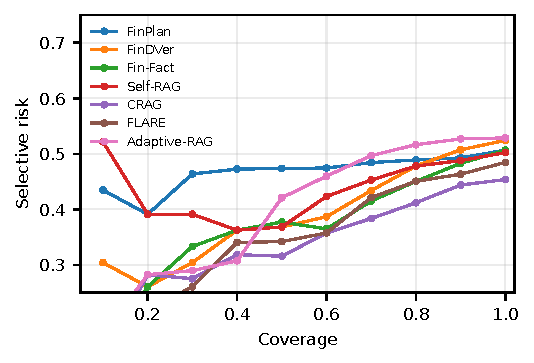
\includegraphics[width=0.78\linewidth]{figures/risk_coverage_named.pdf}
\caption{227条核验样本上的选择性风险-覆盖率曲线。CRAG的AURC最低、选择性准确率最高，FinPlan在平衡准确率和AUROC上更强。}
\label{fig:risk}
\end{figure}

为检验基座依赖性，我们在GLM 5.3 flash上重复六个官方源码适配（模型\texttt{glm-5.3-flash}，温度0，reasoning effort为low，同一三分类适配和检索配方）。FinPlan在平衡准确率（.561）、MCC（.273）、AUROC（.716）和AP（.524）上最好；FinDVer与FinPlan的宏F1并列最高（.485），并在具名基线中取得最好的平衡准确率（.481）、AUROC（.664）、选择性准确率（.605）和AURC（.412）；Fin-Fact的准确率（.542）和MCC（.256）在具名基线中最好。没有单一模型全面占优，说明FinPlan的平衡准确率优势不依赖单一基座。McNemar检验不拒绝任一GLM基线的准确率相等（$p=.28$至$1.00$）；FinPlan的AUROC高于Fin-Fact、Self-RAG、CRAG、FLARE和Adaptive-RAG且区间排除零，但FinDVer的区间包含零。完整结果见附录B表\ref{tab:glm-zh}。\par
为检验开源基座，我们在本地vLLM上部署Qwen3-8B\cite{qwen2025qwen3}（\texttt{qwen3-8b}，关闭thinking，温度0），在同一227条样本上重复六个官方源码适配，所有行均为227条解析样本。FinPlan仍在平衡准确率（.561）、MCC（.273）、AUROC（.716）和AP（.524）上最好；FLARE在具名基线中取得最好的准确率（.537）、宏F1（.500）、选择性准确率（.544）和AURC（.441），但AUROC只有.630。FinDVer、Fin-Fact和Self-RAG在8B规模降到.361/.383/.308准确率和.502/.518/.462 AUROC；McNemar显示它们与FinPlan的准确率差异显著（$p=.007$、$.020$、$<.001$），CRAG、FLARE和Adaptive-RAG则不显著。FinPlan对每个Qwen3行的AUROC差异区间均排除零。完整结果见附录B表\ref{tab:qwen-zh}。\par

\section{校准与标签核验}
在逻辑回归证据模型上，原始概率给出的规划器平均遗憾值为.287、最大为.601，规划器对答案的区间包含零。温度缩放把十个损失配置上的平均遗憾值降到.052，并使规划器对答案的比较在五个种子中的四个区间排除零。规划器在基础损失上仍略差于固定裁决（3.997对3.919）。该校准检验针对结构化基座，不针对DeepSeek共形层。全量标签上，校准后的规划器平均遗憾值为.036、最大为.352，固定策略排序不变。证据模型结果不依赖46条纯文本标签。\par

\section{滚动基准}
表\ref{tab:rolling}报告737条2015年至2025年样本的滚动基准。该集合包含273条主测试样本和464条更早样本，覆盖更早的制度环境。随机森林的准确率为.537、平衡准确率为.503、ECE为.032、选择性准确率为.593；逻辑回归为.487、.535、.092、.501。两者保留了主测试集上的权衡：随机森林准确率和校准误差更好，逻辑回归平衡准确率更高。滚动集使用同一构造，不是新的独立样本。\par
\begin{table}[htbp]
\centering
\caption{按年份滚动的基座检查}
\label{tab:rolling}
\zihao{5}
\begin{tabular}{lcccccc}
\toprule
模型 & $n$ & Acc. & Bal. & F1 & ECE & Sel@50 \\
\midrule
FinPlan（RF） & 737 & .537 & .503 & .498 & .032 & .593 \\
FinPlan（logistic） & 737 & .487 & .535 & .480 & .092 & .501 \\
\bottomrule
\end{tabular}
\end{table}

表\ref{tab:classical-zh}给出经典基座诊断：在校准后的FinPlan logistic与八个标准模型之间，FinPlan的平衡准确率最高（.561），TF-IDF+数值logistic的准确率和宏F1略高（.511/.488）。这说明平衡准确率优势不是只相对于LLM基线成立。\par
\begin{table}[htbp]
\centering
\caption{经典基座诊断（227条核验样本，种子1）；这些不是具名基线，只用于排除模型类别解释}
\label{tab:classical-zh}
\zihao{5}
\setlength{\tabcolsep}{3pt}
\begin{tabular}{lccc}
\toprule
模型 & Acc. & Bal. & Macro F1 \\
\midrule
FinPlan（校准logistic） & .493 & .561 & .485 \\
Logistic & .498 & .549 & .486 \\
HistGradientBoosting & .507 & .454 & .456 \\
随机森林 & .533 & .497 & .492 \\
XGBoost & .485 & .404 & .405 \\
LightGBM & .476 & .437 & .431 \\
CatBoost & .489 & .498 & .470 \\
TF-IDF logistic & .502 & .496 & .484 \\
TF-IDF+数值 logistic & .511 & .516 & .488 \\
\bottomrule
\end{tabular}
\end{table}

\section{真实序贯证据}
\label{sec:sequential-zh}
本节使用真实的业绩公告作为终端证据。数据集的\texttt{outcome.date}是10-Q申报日，但1,005条样本中有993条在同一季度的更早8-K Item 2.02业绩公告中已经公开实际营收；273条测试样本全部有此类8-K。测试样本从截止日到业绩公告的中位间隔为91天。智能体在截止日可以停止（答案、可信集或弃权）、以成本0.1或0.5获取下一家同伴公司的结果、或等待业绩公告（成本2.0加每日延迟成本$\gamma$）。信念模型是以2010—2020年样本训练的时点logistic模型，特征是目标特征、同伴摘要和截止后天数；2021年为验证集，227条2022—2025年核验样本为测试集。策略组合从固定裁决开始，只有当候选策略把验证损失改善至少0.1时才切换。\par
在24个成本单元（6个$\gamma$、2个证据成本、2个结果成本）上，组合在每一个单元都达到oracle最优候选（平均和最大遗憾值均为0）：在8个廉价延迟单元选择始终等待，在16个昂贵单元选择固定裁决。带同伴获取的规划器从未被选中；同伴证据相对于其成本太弱。该结果是决策时间选择的结果，不是规划器优越性的结果。表\ref{tab:sequential-zh}给出4个代表单元。\par
\begin{table}[htbp]
\centering
\caption{真实序贯证据（227条核验测试样本；证据成本0.1，结果成本2.0）}
\label{tab:sequential-zh}
\zihao{5}
\setlength{\tabcolsep}{3pt}
\begin{tabular}{lcccc}
\toprule
$\gamma$ & 固定裁决 & 始终等待 & 规划器 & 选择 \\
\midrule
0.00 & 3.912 & 2.000 & 2.318 & 等待 \\
0.01 & 3.912 & 2.827 & 3.378 & 等待 \\
0.02 & 3.912 & 3.653 & 4.521 & 等待 \\
0.05 & 3.912 & 6.133 & 4.588 & 固定 \\
\bottomrule
\end{tabular}
\end{table}

\section{负结果}
若干负结果属于本文结论的一部分。普通准确率和选择性预测对标签核验不稳健。规划器单独使用时在基础损失下差于固定裁决（3.011对2.932），本文不声称基础损失上的方法优越性。廉价弃权下最优固定策略是始终弃权（2.000），组合选择它，而规划器单独使用为2.035。当前季度锚点在单独预实验中不足以抵消其成本。在另一个时间协议中，oracle-mode预路由的基础损失为3.516，规划器为3.927；在10个配置中两者各赢5个：预路由赢基础、对称、过度厌恶、昂贵弃权和$\alpha=.05$，规划器赢过度乐观、廉价弃权、窄区间、宽区间和$\alpha=.20$。宽度阈值预路由赢5个，规划器赢4个，窄区间为平局。DeepSeek共形结果对掩码敏感，逻辑回归基座不能复现随机森林结果。受控诊断表明模式切换在机制上可行；真实业绩公告实验支持决策时间选择，但同伴证据本身不足以抵消成本（第\ref{sec:sequential-zh}节）。\par

% ==================== 第7章 ====================
\chapter{讨论与局限}
\label{ch:discussion}

\section{结果的含义}
结果支持一个具体的金融证据系统观点：输出契约是决策变量。固定契约在一个损失区域可能最优，在另一个区域可能很差。策略组合是对候选契约的决策规则，其价值来自读取损失和验证证据，而不是来自更强的点预测器。非LLM随机森林使主结果较为干净；DeepSeek共形替代是敏感性分析，不是主证据。\par
调优固定裁决器是强基线。当区间宽度惩罚相对于错误答案代价较小时，它是最优策略；在基础损失下它是需要击败的策略。组合在基础损失下选择它并匹配最优固定策略损失；在廉价弃权下选择弃权；在宽区间下选择规划器。组合的收益不是统一的方法胜利，而是最优固定策略级遗憾值。损失网格是敏感性分析，不是调参集；更换网格会改变绝对损失，但不会改变固定策略遗憾值的排序。\par

\section{新颖性与贡献边界}
本文不提出新的分类器，也不声称训练了更强的通用语言模型。贡献在于把输出模式、决策时间、证据获取和等待统一到一个可检验的决策接口，并给出与该接口匹配的时点基准和决策层证据。相关工作已经分别研究了检索、验证、校准和拒识；本文的窄缺口是这些组件的联合契约，以及在同一损失下比较固定策略、规划器和策略组合。\par
与单一RAG变体相比，本文的差异体现在三个可检验对象上：能力边界表给出各范式的受限维度；三个命题给出固定接口失效的条件；策略组合给出跨损失区域的遗憾值证据。三者共同构成接口层贡献，而不是点预测器的替换。该定位也明确了本文不覆盖的部分：读者评估、答案级金标准和大规模跨市场验证仍需要后续工作。\par

\section{效度威胁}
构念效度方面，本文将“正确输出”操作为结果标签与损失，而不是答案文本质量。真实金融问答还涉及读者理解、引用可追溯性和合规审查，本文没有覆盖。内部效度方面，标签来自自动抽取和XBRL，存在噪声；核验集只排除纯文本标签，不是人工标注金标准。外部效度方面，任务只覆盖营收指引，结论不能直接外推到其他金融陈述、其他语言或其他市场。统计效度方面，主基准只有273条样本，策略组合的置信区间是样本级自助法；确认性种子复现使用同一批样本，不是独立样本。\par
损失权重是建模选择。本文用10个配置检验排序，而不是声称某一组权重是普遍真理。DeepSeek基线可能受到预训练污染，掩码实验只能部分缓解，不能完全排除。随机森林的平衡准确率低于逻辑回归，但其集合决策更好；点预测质量与决策质量并不相同。策略组合的0.15边际是设计选择，本文报告了确认性种子和敏感性结果。\par

\section{落地条件}
若要在真实投研或合规场景部署，至少需要三项补充。第一，人工核验标签和读者评估，建立答案级金标准。第二，接入真实文件检索和引用追踪，使每个可信集成员都可追溯到申报段落。第三，做损失 elicitation，把高估、低估、弃权和延迟的相对代价从业务方处显式获取，而不是使用本文的默认权重。在这些条件满足之前，本文的系统是证据裁决原型，不是投资建议系统，也不应在没有人工复核的情况下自动执行。\par

% ==================== 第8章 ====================
\chapter{结论}
\label{ch:conclusion}
前瞻性金融陈述没有固定的输出契约。系统必须决定何时决策、获取什么证据以及如何回答。本文将输出接口形式化为可信状态上的决策问题，说明固定输出模式在非对称损失下为何只能覆盖部分损失区域，并构建了273条主基准和737条滚动扩展。在227条XBRL核验标签上，证据模型把平衡准确率从.333提高到.564，把宏F1从.220提高到.488。在非LLM随机森林上，损失感知策略组合在10个损失配置中9个达到最优固定策略损失，并在宽区间下取得更低损失（4.340对4.710）。平均遗憾值为$-0.037$，最大遗憾值为0.000；确认性种子复现了宽区间收益和基础损失的精确匹配。\par
六个官方源码适配基线在点预测上各有优势，但没有单一模型全面占优；在DeepSeek、GLM 5.3 flash和Qwen3-8B三个基座上，FinPlan的平衡准确率和AUROC优势均成立。点预测结论与决策层结论必须分开表述。未来工作包括：人工核验标签与读者评估、真实文件检索与引用追踪、损失 elicitation、跨市场和跨语言的时点基准，以及把策略组合扩展到更多候选契约。\par

% ==================== 参考文献 ====================
\clearpage
\addcontentsline{toc}{chapter}{参考文献}
\printbibliography[heading=bibintoc,title={参考文献}]

% ==================== 致谢 ====================
\clearpage
\sufehead{致\quad 谢}
{\zihao{5}\songti
感谢在论文选题、研究设计和写作过程中提供帮助的老师和同学。感谢公开提供SEC申报文件、XBRL数据和相关开源工具的机构与开发者。本文的实验结果和代码均来自可复现的实验脚本；文中错误由作者承担。\par
}

% ==================== 附录 ====================
\appendix
\chapter{命题证明}
\label{app:proofs}
\section{点答案不足}
设$S_t$不是单点集，且错误答案的代价高于集合宽度惩罚。若策略只返回点答案，则在两个与$S_t$一致的后验下，最坏情况风险至少为错误答案代价的一半。可信集在结果不确定时可以把宽度惩罚作为保险，因而在最坏情况下可以更低。该命题说明点答案不是对所有后验都minimax最优，不说明点答案在所有后验下都差。\par
\section{相关性不足}
设相关性分数$s(z,q)$在纤维$\mathcal{F}_r=\{z:s(z,q)=r\}$上为常数，且该纤维包含两个约束不同的证据。只观察$s$的策略无法区分两者，因此在两个世界中采取同一动作，至少在一个世界中选错。若两个世界等先验，错误率至少为$1/2$。\par
\section{预路由不足}
设两个查询有相同的证据前观测，但证据到达后最优模式不同。预路由把相同观测映射到同一模式，因此至少在一个查询上选错。状态依赖规划器可以在证据后分别选择模式，损失差为正。\par

\chapter{复现与补充结果}
\label{app:reproduce}
\section{数据、代码与复现清单}
\label{app:data}
本文的1,005条基准发布为\texttt{paper/\allowbreak data/\allowbreak dataset\_v4.json}（SHA-256
\texttt{\seqsplit{cf24c311806cc15d204b19b8a52c8f3bae6e91bbee563f448cf6643d40923f24}}），
清单为\texttt{paper/\allowbreak data/\allowbreak manifest\_v4.json}，构建规则和许可见
\texttt{paper/\allowbreak data/\allowbreak README.md}。数据文件保留每条样本的SEC链接、声明文本、指引区间、当前季度值、结果和核验来源。代码位于\texttt{scripts/}和\texttt{src/finplan\_rag/}，完整命令见\texttt{paper/reproduce.md}。主策略组合由\path{scripts/analyze_portfolio.py}生成，具名基线由\path{scripts/run_named_baselines.py}生成，逐样本输出、解析标签、可信集和原始响应文本保存在\path{paper/results/}\allowbreak\texttt{deepseek/named/}、\allowbreak\texttt{glm/named/}和\allowbreak\texttt{qwen3/named/}。DeepSeek行使用Anthropic兼容端点和模型标识\texttt{deepseek-flash[1m]}，温度0、关闭thinking、JSON输出，并按提示哈希缓存；该标识是服务商别名而非冻结快照，严格复现需要同一快照或发布的逐样本输出。\par

\begin{table}[htbp]
\centering
\caption{复现清单}
\label{tab:repro}
\zihao{5}
\begin{tabular}{p{0.28\linewidth}p{0.16\linewidth}p{0.46\linewidth}}
\toprule
项目 & 是否发布 & 位置/说明 \\
\midrule
1,005条基准与标签 & 是 & \texttt{paper/\allowbreak data/\allowbreak dataset\_v4.json} \\
数据清单与哈希 & 是 & \texttt{paper/\allowbreak data/\allowbreak manifest\_v4.json} \\
特征、损失、种子 & 是 & \texttt{scripts/}，本文表\ref{tab:lossgrid} \\
组合选择与RF诊断 & 是 & \path{scripts/analyze_portfolio.py} \\
具名基线提示与解析 & 是 & \path{scripts/run_named_baselines.py} \\
逐样本预测与原始文本 & 是 & \path{paper/results/{deepseek,glm,qwen3}/named/} \\
LLM完整响应缓存 & 否（91MB） & 逐样本文件保留解析结果和原文 \\
模型冻结快照 & 否 & 服务商别名\texttt{deepseek-flash[1m]} \\
人工金标准 & 否 & 自动抽取标签；核验集是噪声敏感性 \\
\bottomrule
\end{tabular}
\end{table}

\section{损失配置}
\label{app:lossgrid}
表\ref{tab:lossgrid}列出正文使用的十个损失配置的完整权重。\par

\begin{table}[htbp]
\centering
\caption{十个损失配置}
\label{tab:lossgrid}
\zihao{5}
\setlength{\tabcolsep}{3pt}
\begin{tabular}{lccccccc}
\toprule
配置 & wrong & over & under & miss & width & abstain & alpha \\
\midrule
基础 & 10 & 12 & 8 & 8 & 2 & 5 & .10 \\
对称 & 10 & 10 & 10 & 8 & 2 & 5 & .10 \\
过度厌恶 & 10 & 20 & 5 & 8 & 2 & 5 & .10 \\
过度乐观 & 10 & 5 & 20 & 8 & 2 & 5 & .10 \\
廉价弃权 & 10 & 12 & 8 & 8 & 2 & 2 & .10 \\
昂贵弃权 & 10 & 12 & 8 & 8 & 2 & 10 & .10 \\
窄区间 & 10 & 12 & 8 & 8 & .5 & 5 & .10 \\
宽区间 & 10 & 12 & 8 & 8 & 4 & 5 & .10 \\
$\alpha=.05$ & 10 & 12 & 8 & 8 & 2 & 5 & .05 \\
$\alpha=.20$ & 10 & 12 & 8 & 8 & 2 & 5 & .20 \\
\bottomrule
\end{tabular}
\end{table}

\section{切换边际敏感性}
\label{app:margin}
表\ref{tab:margin}在探索性十种子结果上变化组合切换边际。边际低于0.15时，选择器在过度乐观损失下选择规划器，产生$+0.048$的小正遗憾；0.15及以上避免该切换。宽区间选择和基础匹配在整个范围内不变。\par
\begin{table}[htbp]
\centering
\caption{切换边际敏感性（探索性十种子）}
\label{tab:margin}
\zihao{5}
\begin{tabular}{cccc}
\toprule
边际 & 过度乐观下的选择 & 平均遗憾 & 最大遗憾 \\
\midrule
0.00 & 规划器 & $-.032$ & $+.048$ \\
0.05 & 规划器 & $-.032$ & $+.048$ \\
0.10 & 规划器 & $-.032$ & $+.048$ \\
0.15 & 固定裁决 & $-.037$ & $.000$ \\
0.20 & 固定裁决 & $-.037$ & $.000$ \\
0.30 & 固定裁决 & $-.037$ & $.000$ \\
\bottomrule
\end{tabular}
\end{table}

表\ref{tab:perclass}给出具名基线的逐类精确率、召回率和F1。\par
\begin{table}[htbp]
\centering
\caption{逐类精确率/召回率/F1（227条核验样本）}
\label{tab:perclass}
\zihao{5}
\begin{tabular}{lccc}
\toprule
模型 & Below P/R/F1 & Within P/R/F1 & Above P/R/F1 \\
\midrule
FinPlan（logistic） & .29/.82/.43 & .63/.39/.48 & .63/.47/.54 \\
FinDVer & .27/.09/.14 & .39/.48/.43 & .57/.59/.58 \\
Fin-Fact & .30/.09/.14 & .39/.54/.45 & .63/.58/.60 \\
Self-RAG & .27/.12/.17 & .40/.63/.49 & .69/.51/.59 \\
CRAG & .50/.21/.30 & .45/.56/.50 & .64/.63/.64 \\
FLARE & .50/.12/.20 & .42/.56/.48 & .61/.60/.60 \\
Adaptive-RAG & .38/.09/.15 & .38/.52/.46 & .59/.52/.55 \\
\bottomrule
\end{tabular}
\end{table}

\section{GLM 5.3 flash 基座}
\label{app:glm}
表\ref{tab:glm-zh}在同一227条核验样本上重复六个官方源码适配，基座为GLM 5.3 flash。所有行均为227条解析样本。FinPlan在平衡准确率、MCC、AUROC和AP上最好；FinDVer与FinPlan的宏F1并列最高，并在具名基线中取得最好的平衡准确率、AUROC、选择性准确率和AURC；Fin-Fact的准确率和MCC在具名基线中最好。\par
\begin{table}[htbp]
\centering
\caption{GLM 5.3 flash基座上的官方源码适配基线（227条核验样本，全部解析）。GLM行同样存在预训练污染风险；服务商模型标识不是冻结快照，发布的逐样本输出是此表的精确依据。}
\label{tab:glm-zh}
\zihao{5}
\setlength{\tabcolsep}{2pt}
\begin{tabular}{lcccccccc}
\toprule
模型 & Acc. & Bal. & Macro F1 & MCC & AUROC & AP & Sel@50 & AURC \\
\midrule
FinPlan（logistic） & .493 & .561 & .485 & .273 & .716 & .524 & .526 & .468 \\
FinDVer & .529 & .481 & .485 & .229 & .664 & .469 & .605 & .412 \\
Fin-Fact & .542 & .478 & .478 & .256 & .640 & .436 & .561 & .457 \\
Self-RAG & .485 & .418 & .418 & .165 & .598 & .409 & .561 & .490 \\
CRAG & .498 & .459 & .462 & .168 & .596 & .398 & .526 & .495 \\
FLARE & .515 & .437 & .441 & .178 & .600 & .413 & .596 & .435 \\
Adaptive-RAG & .480 & .400 & .397 & .146 & .566 & .392 & .491 & .511 \\
\bottomrule
\end{tabular}
\end{table}

\section{Qwen3-8B 开源基座}
\label{app:qwen}
表\ref{tab:qwen-zh}在同一227条核验样本上重复六个官方源码适配，基座为本地vLLM部署的开源Qwen3-8B（关闭thinking，温度0）。所有行均为227条解析样本。FinPlan在平衡准确率、MCC、AUROC和AP上最好；FLARE在具名基线中取得最好的准确率、宏F1、选择性准确率和AURC；FinDVer、Fin-Fact和Self-RAG在8B规模明显退化。FinPlan对每个Qwen3行的AUROC差异区间均排除零。\par
表\ref{tab:backbone-zh}汇总三个基座：FinPlan的平衡准确率和AUROC在每个基座上都是最高，官方源码基线只能通过牺牲少数类召回换取准确率或选择性指标。\par
\begin{table}[htbp]
\centering
\caption{三个基座的官方源码适配汇总对比（227条核验样本）。最佳具名基线为该基座上六个方法中的最高值：DeepSeek为CRAG，GLM为FinDVer，Qwen3为FLARE。}
\label{tab:backbone-zh}
\zihao{5}
\begin{tabular}{lcccc}
\toprule
基座 & FinPlan Bal. & 最佳基线 Bal. & FinPlan AUROC & 最佳基线 AUROC \\
\midrule
DeepSeek & .561 & .469（CRAG） & .716 & .689（CRAG） \\
GLM 5.3 flash & .561 & .481（FinDVer） & .716 & .664（FinDVer） \\
Qwen3-8B & .561 & .509（FLARE） & .716 & .630（FLARE） \\
\bottomrule
\end{tabular}
\end{table}
\begin{table}[htbp]
\centering
\caption{Qwen3-8B基座上的官方源码适配基线（227条核验样本，全部解析）。Qwen3行同样存在预训练污染风险，但本地小模型的暴露程度低于API基座。}
\label{tab:qwen-zh}
\zihao{5}
\setlength{\tabcolsep}{2pt}
\begin{tabular}{lcccccccc}
\toprule
模型 & Acc. & Bal. & Macro F1 & MCC & AUROC & AP & Sel@50 & AURC \\
\midrule
FinPlan（logistic） & .493 & .561 & .485 & .273 & .716 & .524 & .526 & .468 \\
FinDVer & .361 & .341 & .231 & -.018 & .502 & .347 & .333 & .650 \\
Fin-Fact & .383 & .358 & .281 & .052 & .518 & .343 & .342 & .615 \\
Self-RAG & .308 & .281 & .207 & -.106 & .462 & .321 & .289 & .675 \\
CRAG & .485 & .454 & .440 & .201 & .590 & .397 & .491 & .499 \\
FLARE & .537 & .509 & .500 & .270 & .630 & .423 & .544 & .441 \\
Adaptive-RAG & .515 & .479 & .487 & .212 & .606 & .415 & .500 & .470 \\
\bottomrule
\end{tabular}
\end{table}

\section{官方源码基线的来源与替换}
\label{app:provenance}
表\ref{tab:provenance-zh}列出六个基线仓库的固定commit、复用的官方组件和替代项。提示模板和决策函数由脚本\texttt{official\_prompts.py}从这些文件加载；逐样本输出、原始响应和提示哈希在\path{paper/results/}\allowbreak\path{official/}。这张表是基线比较的审计边界：这些行是官方源码驱动的适配，不是原系统的未修改运行。\par
\begin{table}[htbp]
\centering
\caption{官方源码基线来源（固定commit）与替换项}
\label{tab:provenance-zh}
\zihao{5}
\setlength{\tabcolsep}{2pt}
\begin{tabular}{p{1.5cm}p{3.4cm}p{4.4cm}p{4.4cm}}
\toprule
方法 & 官方仓库@commit & 复用的官方组件 & 替代项 \\
\midrule
FinDVer & \path{yilunzhao/FinDVer} @ \texttt{e8bb237} & CoT系统提示、文档/声明格式 & 二分类entailment映射为三分类；未运行原retriever/checkpoint \\
Fin-Fact & \path{IIT-DM/Fin-Fact} @ \texttt{b303878} & open-book事实核查提示、claim/\allowbreak evidence格式 & TRUE/\allowbreak FALSE/\allowbreak NEI映射为三分类；未运行图像/训练流程 \\
Self-RAG & \path{AkariAsai/self-rag} @ \texttt{1fcdc42} & instruction/\allowbreak retrieval模板、need-\allowbreak retrieval与relevance critic & selfrag Llama2 critic替换为API critic调用 \\
CRAG & \path{HuskyInSalt/CRAG} @ \texttt{de7c296} & \path{format_prompt}、correct/\allowbreak incorrect/\allowbreak ambiguous动作逻辑 & T5 retrieval evaluator替换为API evaluator \\
FLARE & \path{jzbjyb/FLARE} @ \texttt{ec4b06b} & 低置信度标注函数、主动检索循环结构 & token log-prob替换为自报置信度触发 \\
Adaptive-RAG & \path{starsuzi/Adaptive-RAG} @ \texttt{0c88670} & A/\allowbreak B/\allowbreak C复杂度语义与路由动作 & T5 classifier未发布，改用API zero-shot分类器 \\
\bottomrule
\end{tabular}
\end{table}

\end{document}
